\subsection{Ütközések feloldása}

%14
\begin{frame}
  \begin{itemize}
    \item Ha több előírás is vonatkozik ugyanannak az objektumnak a formázására, elsőként a forrás prioritása dönt (csökkenő sorrendben):
    \begin{enumerate}
      \item soron belüli formázások
      \item külső és belső (\texttt{<link>}, \texttt{<style>} elemek) formázások
      \item böngésző alapértelmezése
    \end{enumerate}
    \item Ha forrás alapján nem lehet különbséget tenni, megvizsgálják a \emph{specifikusságot}.
    \item Ha ez sem segít, a később betöltött szabály felülírja a korábbit.
  \end{itemize}
  
\end{frame}

%15
\begin{frame}
  \begin{exampleblock}{\textattachfile{utkozes1.html}{utkozes1.html}}
    \scriptsize
    \lstinputlisting[style=HTML,linerange={6-13},numbers=left,firstnumber=6]{utkozes1.html}
  \end{exampleblock}
  \begin{columns}[T]
    \column{0.6\textwidth}
      \begin{exampleblock}{\textattachfile{utkozes1.css}{utkozes1.css}}
        \scriptsize
        \lstinputlisting[style=HTML,numbers=left,firstnumber=1]{utkozes1.css}
      \end{exampleblock}
    \column{0.3\textwidth}
      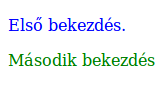
\includegraphics[width=.66\textwidth]{utkozes1.png}
  \end{columns} 
\end{frame}

%16
\begin{frame}
  \begin{exampleblock}{\textattachfile{utkozes2.html}{utkozes2.html}}
    \scriptsize
    \lstinputlisting[style=HTML,linerange={6-13},numbers=left,firstnumber=6]{utkozes2.html}
  \end{exampleblock}
  \begin{columns}[T]
    \column{0.6\textwidth}
      \begin{exampleblock}{\textattachfile{utkozes1.css}{utkozes1.css}}
        \scriptsize
        \lstinputlisting[style=HTML,numbers=left,firstnumber=1]{utkozes1.css}
      \end{exampleblock}
    \column{0.3\textwidth}
      
\includegraphics[width=.66\textwidth]{utkozes2.png}
  \end{columns} 
\end{frame}

%_
\begin{frame}
  Specifikusság meghatározása
  \begin{enumerate}
    \renewcommand{\theenumi}{\Alph{enumi}}
    \item = 1, ha a stílus a \texttt{style} attribútumban található, egyébként 0\\(pl. \texttt{<p style="color: red;">...</p>})
    \item = a szelektorban lévő ID attribútumok száma (pl. \texttt{\#bekezdes})
    \item = a szelektorban lévő osztályok, attribútumok és látszólagos osztályok száma\\(pl. \texttt{.bekezdes}, \texttt{a[target="\_blank"]}, \texttt{a:hover})
    \item = az elemnevek és látszólagos elemek száma (pl. \texttt{p}, \texttt{p::first-line})
  \end{enumerate}
  Az univerzális szelektor (\texttt{*}) és ami ebből származik (pl. \texttt{body *}) 0 specifikusságú.
\end{frame}

%_
\begin{frame}
  \begin{center}
    \begin{tabular}{lllll}
    Szelektor & B & C & D & Specifikusság \\ \hline
    \texttt{*} & 0 & 0 & 0 & 0\\
    \texttt{p} & 0 & 0 & 1 & 1\\
    \texttt{div p} & 0 & 0 & 2 & 2\\
    \texttt{ul ol + li} & 0 & 0 & 3 & 3\\
    \texttt{h1 + *[title]} & 0 & 1 & 1 & 11\\
    \texttt{ul ol li.voros} & 0 & 1 & 3 & 13\\
    \texttt{li.voros.szint} & 0 & 2 & 1 & 21\\
    \texttt{\#oszlopfej} & 1 & 0 & 0 & 100
    \end{tabular}
  \end{center}
\end{frame}
